\documentclass[runningheads]{llncs}
\usepackage{amssymb}
\setcounter{tocdepth}{3}
\usepackage{graphicx,epsfig}
\usepackage{algorithmic}
\usepackage{listings}
\usepackage{rotating}
\usepackage{subfig}
\usepackage[boxed]{algorithm2e}

%%%%

\usepackage{color}
\usepackage{alltt}
\usepackage{verbatim}
\usepackage{url}
\usepackage[latin1]{inputenc}
%\usepackage[spanish]{babel}

%%

\usepackage{url}
\urldef{\mailsa}\path|pgarcia@atc.ugr.es|



\newcommand{\keywords}[1]{\par\addvspace\baselineskip
\noindent\keywordname\enspace\ignorespaces#1}

\lstset{
basicstyle=\ttfamily, %\scriptsize, QUITAR LA COMA DE TTFAMILY SI DESCOMENTAS
language=c++,
frame=single,
stringstyle=\ttfamily,
showstringspaces=false
}

\begin{document}
 %\pagestyle{empty} %ESTO QUITA LOS NUMEROS DE PAGINA
\mainmatter  % start of an individual contribution

% DUDAS DE LA MUERTE, A VER QUIEN ME RESPONDE:
% DIFERENCIAS ENTRE BOT Y AGENT


% first the title is needed
\title{Difference of tree maximum depth in Genetic Programming to
  generate competitive agents for RTS games}
% Ein? No entiendo nada. �Quieres vender la diferencia de profundidad
% m�xima?  - JJ FERGU: Inicialmente, y sin tener resultados todav�a

% a short form should be given in case it is too long for the running head
\titlerunning{Difference of tree maximum depth in GP for RTS games}
\author{P. Garc\'ia-S\'anchez, A. Fern\'andez-Ares, A. M. Mora,
  P. A. Castillo and J.J. Merelo}

%Doble ciego!!!!! - JJ FERGU: Lo s�, es para ver quien participa.
 
%

\authorrunning{P. Garc\'ia-S\'anchez et al.}

% (feature abused for this document to repeat the title also on left hand pages)
% the affiliations are given next; don't give your e-mail address
% unless you accept that it will be published

\institute{Dept. of Computer Architecture and Technology and CITIC-UGR, University of Granada, Spain 
\mailsa}




%\toctitle{BLABLABLA}
%ES ANONIMO????
% S�! - JJ FERGU: que ya lo sab�a, esto es del primer Evostar que envi� hace mil a�os y conserva los comentarios que escrib� xDD
%\tocauthor{Authors' Instructions}
\maketitle


\begin{abstract}

This work presents the results obtained from comparing ... Results
show that 

% Por eso es por lo que ten�is que escribir el abstract antes que
% nada; para afinar el t�tulo y tener claro qu� es lo qeu quer�is
% probar. FERGU: Si empiezo a escribir el art�culo sin tener resultados tendr� que esperar que las ejecuciones terminen para decir algo... Por ahora estoy escribiendo al principio el SOA y la descripci�n de lo que se est� ejecutando, a falta de que termine.

\end{abstract}


% En el GPBot tienes que hacer �nfasis en que las estrategias probadas
% hasta ahora en este juego son tan buenas como la estrategia original
% que parametrizan; 
% FERGU: No me he enterado de esto
% GPBot te permite no s�lo conseguir estrategias
% mejores, sino descubrirlas. En los resultados tienes que hacer
% �nfasis no s�lo en lo obtenido, sino tambi�n en qu� significan las
% estrategias, c�mo juegan; tendr�s que ponerlas a jugar a ver qu� pasa.
% FERGU: esa era la idea, pero hasta que no terminen las 4 ejecuciones que est�n ejecutandose que duran 4 d�as...


\section{Introduction}
\noindent 

Real Time Simulators (RTS) are a type of videogame that... 



One of the most used games for study computational intelligence in RTS
is {\em Planet Wars}
\cite{Lara2013mapgenerator,Mora2012Genebot,FernandezAres2012adaptive}
% Recordad doble ciego - JJ
 because it is a simple RTS that defines a ... %esto no corresponde al
                                %estado del arte, sino a la
                                %introducci�n - JJ FERGU: OK, movido arriba
 Although it has been described in previous works, we summarize saying that the objective of the player is to conquer enemy and neutral planets in a space-like simulator. Each player has planets that produce ships depending of a growth-rate and the player must send this ships to other planets (literally, crashing towards the planet) to conquer them. A player win if is the owner of all the planets. As requirements, each second a decission has to be made (turn), and no memory about the previous turns must be used. Figure \ref{fig:naves} show a screen capture of the game. 

\begin{figure}
\begin{center}
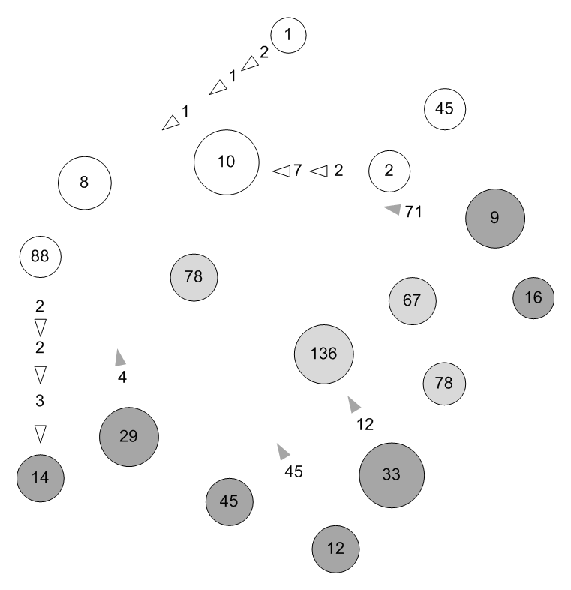
\includegraphics[scale=0.8]{naves.eps}
\end{center} 
\caption{Example of execution of the Player Wars game. White planets and ships are owned by the player and dark gray ones are controlled by the enemy. Clear gray are neutral planets (not invaded).}
\label{fig:naves}
\end{figure}


In this work we use Genetic Programming (GP) to obtain agents that play
Planet Wars game. The objective of GP is to create functions or programs to solve determined problems. Individual representation is usually in form of a tree, formed by operators (or {\em primitives}) and variables ({\em terminals}). These sets are usually fixed and known. The genome size is, therefore, variable, but the maximum size (depth) of the individuals is usually fixed, to avoid high evaluation costs. GP has been used to evolve LISP (LISt Processing) programs \cite{Koza1990Tools}, or XSLT (eXtensible Stylesheet Language Transformations) scripts \cite{Garcia2008XSLT}, among others.

% Breve
                                % explicaci�n de GP, no es un congreso
                                % exclusivo de eso y no es tan
                                % conocido como GA en general - JJ
                                % FERGU: OK 
We try to solve the next questions: 
\begin{itemize}
\item Can a tree-generated behaviour of an agent defeat a hand-coded one whose parameters have been also optimized?
\item Can this agent beats a more complicated oponent that is adapted to the environment?
\item How does the maximum depth affects the results?
\end{itemize}

The rest of the work is structured as follows: after the state of the art, the description of our agent is presented in Section \ref{sec:agent}. Then, the experimental setup conduced with the EA are showed (Section \ref{sec:experiments}). Finally, results, conclusions and future works are discussed.


%%%%%%%%%%%%%%%%%%%%%%%%SEC SOA
\section{State of the art}
\label{sec:soa}

RTS games  (see \cite{Lara2013review} for a survey). %surey o survey ? FERGU: no lo hab�a metido aun en el bibtex, cambio a review

Among other techniques, Evolutionary Algorithms (EAs) have been widely used in computational intelligence in RTS games \cite{Lara2013review}. For example, for parameter optimization \cite{Esparcia10FPS}, learning \cite{Kenneth2005neuroevolution} or content generation \cite{Mahlmann2012MapGeneration}. 

One of these types, Genetic Programming, has been proved as a good tool for developing strategies in games achieving results comparable to human, or human-based, competitors \cite{Sipper2007gameplaying}, and achieving higher ranking than solvers produced by other techniques or even beating high-ranking humans \cite{Elyasaf2012FreeCell}. GP has also been used in different kind of games, such as board-games \cite{Benbassat2012Reversi}, or (in principle) simpler games such as Ms. Pac-Man \cite{Brandstetter2012PacMan} and Spoof \cite{Wittkamp2007spoof} and even in modern video-games such as First Person Shoothers (FPS) (for example, Unreal \cite{Esparcia2013GPunreal}).

%We have experimented with this game in previous works. 
Planet Wars, the game we are going to use in this work, has been used as experimental environment in other works. For example, in
\cite{Mora2012Genebot} the authors programmed the behaviour of a bot with a decission tree of 3 levels. Then, the values of these rules were optimized using a genetic algorithm to tune the strategy rates and percentages.  % ein????? - JJ - FERGU: re-escrito.
  Results showed a good performance confronting with other bots
  provided by the Google AI Challenge. %In our next work
  In their next work
  \cite{FernandezAres2012adaptive} they improved this agent optimizing
  in different types of maps and selecting the set of optimized
  parameters depending of the map where the game was taking place,
  using a tree of 5 levels. These results outperformed the previous
  version of the bot with 87\% of victories. % DOBLE CIEGO!!!! - jj - FERGU: que yaaaaa xD

In this paper we use Genetic Programming to create the decission tree,
instead of using our own gaming experience to model it, and compare
this agent with the two presented before.  % POR FAVOR, meted a Paloma a bordo para
                             % que revise el ingl�s - JJ



\section{Proposed Agent}
\label{sec:agent}


The proposed agent receives a tree to be executed. The generated tree
is a binary tree of expressions formed by two different types of nodes:

\begin{itemize}
\item {\em Decission}: a logical expression formed by a variable, a less than operator ($<$), and a number between 0 and 1. They are the equivalent to the ``primitives'' in the field of GP.
\item {\em Action}: the leaves of the the tree (therefore, the ``terminals''). Each decission is the name of the method to call that indicates to which planet send a percentage of available ships (from 0 to 1) from the planet that executes the tree. 
\end{itemize}

The different variables for the decissions are:

\begin{itemize}
\item {\em myShipsEnemyRatio}: Ratio between the player's ships and enemy's ships.
\item {\em myShipsLandedFlyingRatio}: Ratio between the player's landed and flying ships.
\item {\em myPlanetsEnemyRatio}: Ratio between the number of player's planets and the enemy's ones.
\item {\em myPlanetsTotalRatio}: Ration between the number of player's planet and total planets (neutrals and enemy included)-
\item {\em actualMyShipsRatio}: Ratio between the number of ships in the specific planet that evaluates the tree and player's total ships.
\item {\em actualLandedFlyingRatio}: Ratio between the number of ships landed and flying from the specific planet that evaluates the tree and player's total ships.
\end{itemize}

The decission list is:
% �De d�nde hab�is sacado esto? Tambi�n tienen una cierta estrategia
% presupuesta: que hay que elegir objetivos, por ejemplo - JJ FERGU: me lo he inventado yo, son las decisiones que puede tomar el bot
\begin{itemize}
\item {\em Attack Nearest (Neutral|Enemy|NotMy) Planet}: The objective is the nearest planet.
\item {\em Attack Weakest (Neutral|Enemy|NotMy) Planet}: The objective is the planet with less ships.
\item {\em Attack Wealthest (Neutral|Enemy|NotMy) Planet}: The objective is the planet with higher lower rate.
\item {\em Attack Beneficious (Neutral|Enemy|NotMy) Planet}: The objective is the planet more beneficious, that is the one with growth rate divided by the number of ships.
\item {\em Attack Quickest (Neutral|Enemy|NotMy) Planet}: The objective is the planet with higher facility to conquest: the lowest product between the distance from the planet that executes the tree and the number of the ships in the objective planet.
\item {\em Attack (Neutral|Enemy|NotMy) Base}: The objective is the planet with more ships (that is, the base).
\item {\em  Attack Random Planet}.
\item {\em Reinforce Nearest Planet}: Reinforce the nearest player's planet to the planet that executes the tree.
\item {\em Reinforce Base}: Reinforce the player's planet with higher number of ships.
\item {\em Reinforce Wealthest Planet}: Reinforce the player's planet with higher grown rate.
\item {\em Do nothing}.


\end{itemize}

An example of a possible tree is shown in Figure \ref{fig:java}. This example tree has a total of 5 nodes, with 2 decissions and 3 actions, and a depth of 3 levels.

\begin{figure}[tb] 
\begin{center}
\begin{lstlisting}
if(myShipsLandedFlyingRatio<0.796)
	if(actualMyShipsRatio<0.201)
		attackWeakestNeutralPlanet(0.481);
	else
		attackNearestEnemyPlanet(0.913);
else
	attackNearestEnemyPlanet(0.819);
\end{lstlisting}
\end{center}
\caption{Example of a generated Java tree.}
\label{fig:java}
\end{figure}

The bot behaviour is explained in Algorithm \ref{alg:turn}.

\begin{algorithm}
\SetAlgoLined
%\KwData{this text}
%\KwResult{how to write algorithm with \LaTeX2e }

\emph{At the beginning of the execution the agent receives the tree}\;
tree$\leftarrow$ readTree()\;
\While{game not finished}{
	\tcp{starts the turn}
	calculateGlobalPlanets();\tcp{e.g. Base or Enemy Base}\
	calculateGlobalRatios();\tcp{e.g. myPlanetsEnemyRatio}\
	\ForEach{p in PlayerPlanets}{
		calculateLocalPlanets(p);\tcp{e.g. NearestNeutralPlanet to p}\
		calculateLocalRatios(p);\tcp{e.g actualMyShipsRatio}\
		executeTree(p,tree);\tcp{Send a percentage of ships to destination}\
	}
	
}

\caption{Pseudocode of the proposed agent. The tree is fixed during all the agent's execution}
\label{alg:turn}
\end{algorithm}




%\COMMENT {In each turn}
%\LOOP
	
%	\STATE calculateGlobalPlanets()
%	\COMMENT{{\em for example Base, Enemy Base...}}
%	\STATE calculateGlobalRatios ()
%	\COMMENT {{\em for example myPlanetEnemyRatio, myShipsEnemyRatio...}}
%		\FOR{each Planet: p}
%			\STATE calculateLocalPlanets (p)
%			\COMMENT{{\em for example NearestNeutralPlanet to planet p}}
%			\STATE calculateLocalRatios (p)
%			\COMMENT{{\em for example actualMyShipsRatio}}
%			\STATE executeTree(p,tree)
%			\COMMENT{{\em Send a percentage of the ships to another planet}}
%		\ENDFOR
%\ENDLOOP




\section{Experimental Setup}
\label{sec:experiments}

To generate the tree we have used a Genetic Programming Algorithm. Evolutionary operators used are the sub-tree crossover and 1-node mutation. The choice is suggested by other researchers that have used these operators obtaining good results \cite{Esparcia2013GPunreal}. In our case the mutation randomly changes the decission of a node or mutate the value with an step-size of 0.25. Each configuration is executed 30 times, with a population of 32 individuals and a 2-tournament selector for a pool of 16 parents.

To test each individual during the evolution a battle with a previously created bot is performed in 5 different (but representative) maps provided by Google. The fitness used is a hierarchichal one previously used by other researchers in \cite{Mora2012Genebot}. In our case, an individual is better than another if it wins in more maps. In case of equality of victories, then the individual with more turns to be defeated (i.e. it is stronger) is considered better. The maximum fitness is, therefore 5 victories and 0 turns. Also, as proposed by \cite{Mora2012Genebot}, and due to the noisy fitness effect, in every generation all individuals are re-evaluated.


Two publicly available bots have been chosen for our experiments\footnote{Both can be downloaded from \url{http://github.com/METEAQUILAURL}}. The first bot to confront is {\em GeneBot}, proposed in the work \cite{Mora2012Genebot}. This bot was trained using a GA to optimize the 8 parameters that conforms a set of hand-made rules. The other chosen bot is an advanced version of the previous one, called {\em ExGenebot} presented in \cite{FernandezAres2012adaptive}. This bot outperformed Genebot widely. ExGenebot bot analyses the distribution of the planets of the map to chose a previously optimized set of parameters. 

After executing our algorithm without tree limitation in depth we also have executed with the lower and average levels obtained for the best individuals: 3 and 7, respectively, to study if this number has any effect in the results.   Table \ref{tab:parameters} summarizes all the parameters used.

\begin{table}
\begin{center}
\begin{tabular}{|c|c|}
\hline
{\em Parameter Name} & {\em Value} \\\hline
Population size & 32 \\\hline
Crossover type & Sub-tree crossover \\ \hline
Crossover rate & 0.5\\ \hline
Mutation  & 1-node mutation\\ \hline
Mutation step-size & 0.25 \\ \hline
Selection & 2-tournament \\ \hline
Replacement & Steady-state\\ \hline
Stop criterion & 50 generations \\ \hline
Maximum Tree Depth & 3, 7 and unlimited \\ \hline
Runs per configuration & 30 \\ \hline
Evaluation & Playing versus Genebot \cite{Mora2012Genebot} and ExGenebot \cite{FernandezAres2012adaptive} \\ \hline
Maps used in each evaluation & \\ \hline
\end{tabular}
\caption{Parameters used in the experiments.}
\label{tab:parameters}
\end{center}
\end{table}

After all the executions we have evaluated all the obtained best individuals in all runs confronting to the bots in a larger set of maps (the 100 maps provided by Google) to study the behaviour of the algorithm and how good are the obtained bots in maps that have not been used for training.

The used framework is OSGiLiath, a service-oriented evolutionary framework. The generated tree is compiled in real-time and injected in the agent's code using Java CAssist library. All the source code used in this work is available under a LGPL V3 License in \url{http://www.osgiliath.org}.

\section{Results}

Table \ref{tab:results} summarizes all the obtained results of the execution of our EA. This table also shows the average age, depth and number of nodes of the best individuals obtained and also the average population at the end of the run. The average turns columns are calculated only taking into account the individuals with lower victories than 5, because this number is 0 if they have win the five battles.

%\begin{table*}
%\centering{\scriptsize
%\begin{tabular}{|c|c|c|c|c|c|c|c|c|c|c|} \hline
%  & \multicolumn{2}{|c|}{Best Fitness (avg.)} & \multicolumn{2}{|c|}{Average Fitness (avg.)} & \multicolumn{2}{|c|}{Depth} & \multicolumn{2}{|c|}{Nodes} & \multicolumn{2}{|c|}{Age} \\ \hline
%\multicolumn{11}{|c|}{Versus Genebot} \\ \hline
%Depth & Victories & Turns   & Victories & Turns   & Best & Population & Best  & Population  & Best   & Population \\ \hline
%3      & 4.933 $\pm$ 0.25    & 244.5 $\pm$  54.44 & 4.486 $\pm$ 0.52  & 130.77  $\pm$ 95.81 &   3  $\pm$ 0 & 3          $\pm$ 0 & 7  $\pm$ 0 & 7        $\pm$ 0 & 8.133 $\pm$ 3.95 & 4.297  $\pm$ 3.027  \\ \hline
%Unlimited & 4,9 $\pm$ 0.30   & 266,667 $\pm$ 40.42 & 4,711  $\pm$ 0.45  &190,346 $\pm$102.92 & 6,933 $\pm$ 4.05 & 7,353  $\pm$ 3.11   & 22,133 $\pm$ 22.21&  21,418 $\pm$ 13.81   & 5,066 $\pm$ 2.11 & 3,0927 $\pm$ 1.27 \\ \hline

%\multicolumn{11}{|c|}{Versus ExGenebot} \\ \hline
%3 & 4.133 $\pm$ 0.50 & 221.625 $\pm$ 54.43 &  3.541 $\pm$ 0.34  & 200.086 $\pm$ 50.79 & 3 $\pm$ 0 & 3 $\pm$ 0 & 7 $\pm$ 0 & 7 $\pm$ 0 & 4.266 $\pm$  5.01 & 3.706 $\pm$ 0.58 \\ \hline
%7 & 4.2 $\pm$ 0.48  & 163.667  $\pm$ 106.38  & 3.689  $\pm$ 0.37  & 184.076  $\pm$ 57.02  & 5.2 $\pm$ 1.84 & 5.216  $\pm$ 0.92  & 12.6  $\pm$ 6.44  & 13.05  $\pm$ 3.92   & 4.133  $\pm$ 4.26  & 3.727 $\pm$ 0.62 \\ \hline
%Unlimited & 4.4 $\pm$ 0.56 & 123.533 $\pm$ 112.79 & 4.043 $\pm$ 0.38 & 159.094 $\pm$ 61.84 & 6.966 $\pm$ 4.44 & 6.522 $\pm$ 1.91 & 18.466 $\pm$ 15.46 &  16.337 $\pm$ 7.67 &  4.7 $\pm$ 4.72 & 3.889 $\pm$ 0.71  \\ \hline


%\end{tabular}
%\caption{Average results obtained from each configuration. Each one has been tested 30 times.}
%\label{tabcomputers}
%}
%\end{table*}

\begin{table*}
\centering{\scriptsize
\begin{tabular}{|c|c|c|c|c|} \hline
\multicolumn{5}{|c|}{Versus Genebot} \\ \hline
    \multicolumn{2}{|c|}{}    &  Depth 3                & Depth 7                &    Unlimited  Depth    \\ \hline  
Best Fitness  & Victories     &   \textbf{4.933} $\pm$ 0.25       &  4.83 $\pm$ 0.53       &    4,9     $\pm$ 0.30  \\ \hline  
              & Turns         &  244.5 $\pm$  54.44     &  466   $\pm$ 205.44    &    266,667 $\pm$ 40.42 \\ \hline  
Population Ave. Fitness  & Victories     &   \textbf{4.486}$\pm$ 0.52 & 4.43 $\pm$ 0.07   &    4,711   $\pm$ 0.45  \\ \hline  
              & Turns         &  130.77$\pm$ 95.81      &  139.43 $\pm$ 196.60   &    190,346 $\pm$ 102.92\\ \hline  
Depth         & Best          &  3     $\pm$ 0          & 5.2 $\pm$ 1.78         &    6,933   $\pm$ 4.05  \\ \hline  
              & Population    &  3  $\pm$ 0             & 5.267 $\pm$ 1.8        &    7,353   $\pm$ 3.11  \\ \hline  
Nodes         & Best          &  7     $\pm$ 0          &   13.667 $\pm$ 7.68    &    22,133  $\pm$ 22.21 \\ \hline  
              & Population    &  7     $\pm$ 0          & 13.818 $\pm$ 5.86      &    21,418  $\pm$ 13.81 \\ \hline  
Age           & Best          &  \textbf{8.133} $\pm$ 3.95       & 5.467 $\pm$ 2.95       &    5,066   $\pm$ 2.11  \\ \hline  
              & Population    &  \textbf{4.297} $\pm$ 3.027      & 3.247 $\pm$ 0.25       &    3,092   $\pm$ 1.27  \\ \hline
   \multicolumn{5}{|c|}{Versus ExGenebot} \\ \hline             
 \multicolumn{2}{|c|}{}        &  Depth 3                & Depth     7            &   Unlimited Depth     \\ \hline  
Best Fitness  & Victories     &   4.133   $\pm$ 0.50    & 4.2      $\pm$ 0.48    &   \textbf{4.4}     $\pm$ 0.56  \\ \hline 
              & Turns          &  221.625 $\pm$ 54.43   & 163.667  $\pm$ 106.38  &   123.533 $\pm$ 112.79\\ \hline 
Population Ave. Fitness  & Victories      &  3.541   $\pm$ 0.34    & 3.689    $\pm$ 0.37    &   \textbf{4.043}   $\pm$ 0.38  \\ \hline 
              & Turns          &  200.086 $\pm$ 50.79   & 184.076  $\pm$ 57.02   &   159.094 $\pm$ 61.84 \\ \hline  
Depth         & Best           &  3       $\pm$ 0       & 5.2      $\pm$ 1.84    &   6.966   $\pm$ 4.44  \\ \hline 
              & Population     &  3       $\pm$ 0       & 5.216    $\pm$ 0.92    &   6.522   $\pm$ 1.91  \\ \hline 
Nodes         & Best           &  7       $\pm$ 0       & 12.6     $\pm$ 6.44    &   18.466  $\pm$ 15.46 \\ \hline  
              & Population     &  7       $\pm$ 0       & 13.05    $\pm$ 3.92    &   16.337  $\pm$ 7.67  \\ \hline 
Age           & Best           &  4.266   $\pm$ 5.01    & 4.133    $\pm$ 4.26    &   \textbf{4.7}     $\pm$ 4.72  \\ \hline 
              & Population     &  3.706   $\pm$ 0.58    & 3.727    $\pm$ 0.62    &   \textbf{3.889}   $\pm$ 0.71  \\ \hline  


\end{tabular}
\caption{Average results obtained from each configuration. Each one has been tested 30 times.}
\label{tab:results}
}
\end{table*}

The second experiment results are shown in Table \ref{tab:allmaps}. In this experiment we have confronted the 30 bots obtained in each configuration again with Genebot and ExGenebot but in the 100 maps provided by Google. This table shows how the bots obtained using GP wins more times. It can be seen that it is dificult to beat the adapatative bot, because it is using a map-detection mechanism. BLABLABLA. Note that, confronting with ExGenebot, even obtaining individuals with maximum fitness (5 victories) that have been kept in the population several generations cannot be representative of a extremely good bot in a wider set of maps. 

\begin{table*}
\centering{\scriptsize
\begin{tabular}{|c|c|c|c|c|c|c|} \hline
                         
Configuration     &    Average maps won  &    Average turns     \\ \hline
                   \multicolumn{3}{|c|}{Versus Genebot}    \\ \hline
 Depth 3          &                      &                 \\ \hline
 Depth 7          &                      &                 \\ \hline
 Unlimited Depth  &                      &                 \\ \hline
       \multicolumn{3}{|c|}{Versus ExGenebot}                         \\ \hline              
 Depth 3          &   52.367 $\pm$ 13.39 & 9565.667 $\pm$ 5833.60 \\ \hline
 Depth 7          &   58.867 $\pm$ 7.35  & 7389.535 $\pm$ 3574.26 \\ \hline
 Unlimited Depth  &   56 $\pm$ 11.52     & 8247.967 $\pm$ 4133.72 \\ \hline 

\end{tabular}


\caption{Results confronting the 30 best bots attained from each configuration in the 100 maps each.}
\label{tab:allmaps}
}
\end{table*}
 
\section{Conclusions}
\label{sec:conclusion}

This work presents a Genetic Programming algorithm that generates agents for playing Planet Wars game. A number of possible actions to perform and decission variables have been presented. We have used two competitive bots available in the literature (Genebot and ExGenebot) to use to set the fitness of the generated individuals. Three different tree maximum depths have been used: 3, 7 and unlimited. Results show that best individuals outperforms these agents during the evolution in all configurations. We also have tested our agents with a larger set of maps not used for evaluation, obtaining results equivalent or betters that the previous agents.

In future work, other rules will be added to our algorithm (for example, the ones that analyse the map, as the ExGenebot does). Other games used in the area of computational intelligence in videogames, such as Unreal or SuperMario will be tested.

\bibliographystyle{splncs}
\bibliography{gpbot}

\end{document}

